\section{排版数学公式}
这个章节主要介绍的是\LaTeX{}的数学排版公式的问题,因为\LaTeX{}的数学排版公式是其最大的优势,所以这里单独开一个章节来介绍。

\subsection{AMS宏集}
在介绍数学排版之前,首先要介绍的是AMS宏集,因为AMS宏集是\LaTeX{}数学排版的基础,所以这里先做一个简单的介绍。
AMS宏集是美国数学学会(American Mathematical Society)开发的一组\LaTeX{}宏包,用于排版数学公式,它提供了一系列的命令和环境,用于排版数学公式,例如\texttt{align}、\texttt{gather}、\texttt{cases}等等。
AMS宏集的官方文档可以通过\href{https://ctan.org/pkg/amsmath}{https://ctan.org/pkg/amsmath}获取到。
其中核心是\texttt{amsmath}宏包,它提供了一系列的命令和环境,用于排版数学公式。
此外,AMS宏集还提供了一些额外的宏包,例如\texttt{amssymb}、\texttt{amsfonts}、\texttt{amsthm}等等,这些宏包提供了一些额外的命令和环境,用于排版数学公式。
\subsection{行内公式与行间公式}
\LaTeX{}中的数学公式有两种形式,一种是行内公式,一种是行间公式。
行内公式是指在正文中插入数学公式,例如$E=mc^2$,行间公式是指单独的一行显示数学公式,例如我们这里写出了一个行间公式,麦克斯韦方程组:

\begin{equation}
    \begin{aligned}
        \nabla \cdot \mathbf{E} & = \frac{\rho}{\varepsilon_{0}} \\
        \nabla \cdot \mathbf{B} & = 0 \\
        \nabla \times \mathbf{E} & =-\frac{\partial \mathbf{B}}{\partial t} \\
        \nabla \times \mathbf{B} & = \mu_{0} \mathbf{J}+\mu_{0} \varepsilon_{0} \frac{\partial \mathbf{E}}{\partial t}
    \end{aligned}
\end{equation}

积分形式:
\begin{equation}
    \begin{cases}
        \displaystyle\oint_{l}\mathbf{H}\cdot{d}\mathbf{l}&=\displaystyle\iint_\mathbf{S}J\cdot{d}\mathbf{S}+\displaystyle\iint_{S}\dfrac{\partial\mathbf{D}}{\partial{t}}\cdot{dS}\\
        \displaystyle\oint_{l}\mathbf{E}\cdot{d}\mathbf{l}&=-\displaystyle\iint_{S}\dfrac{\partial\mathbf{B}}{\partial{t}}\cdot{d}\mathbf{S}\\
        \displaystyle\oint_{S}\mathbf{B}\cdot{d}\mathbf{S}&=0\\
        \displaystyle\oint_{S}\mathbf{D}\cdot{d}\mathbf{S}&=\displaystyle\iiint_\mathbf{V}\rho{d}\mathbb{V}
    \end{cases}
\end{equation}

再举一个例子,这里列举了薛定谔方程的写法,使用行间公式写出来如下所示:
\begin{equation}
    i \hbar \frac{\partial}{\partial t} \Psi(\mathbf{r}, t)=\left[\frac{-\hbar^{2}}{2 \mu} \nabla^{2}+V(\mathbf{r}, t)\right] \Psi(\mathbf{r}, t)
\end{equation}

详细的教程可以参考上一个章节提及过的学习网站,这里不再过多赘述。
\subsection{画表}
三线表画法:底部和顶部的线条为1.5pt,中间的线条为0.75pt,如表\ref{tab:heightweight}所示。

\begin{table}[!htp]
    \newcolumntype{L}{X}
    \newcolumntype{C}{>{\centering \arraybackslash}X}
    \newcolumntype{R}{>{\raggedright \arraybackslash}X}
    \centering
    \caption{某校学生身高体重样本}
    \label{tab:heightweight}
    \begin{tabularx}{0.9\textwidth}{CCCC}
       \toprule[1.5pt]
        序号&年龄&身高&体重\\
        \midrule[0.75pt]
        1&14&156&42\\
        2&16&158&45\\
        3&14&162&48\\
        4&15&163&50\\
        \midrule[0.75pt]
        %\cmidrule{2-4}
        平均&15&159.75&46.25\\
        \bottomrule[1.5pt]
    \end{tabularx}
\end{table}

表\ref{tab:some_products_datasets}所示是一个简单的双并排表的一个画法。
\begin{table}[htp!]
    \centering
    \caption{某行业产量与生产费用的数据}
    \label{tab:some_products_datasets}
    \newcolumntype{Y}{>{\centering\arraybackslash}X}
    \newcolumntype{Z}{!{\vline}@{\color{white}\vrule width \doublerulesep}!{\vrule}}%自定义列格式(双线)
    \begin{tabularx}{0.94\textwidth}{c|c|YZc|c|Y}
        \Xhline{0.9pt}
        企业编号&	产量(台)&生产费用(万元)&企业编号&产量(台)&生产费用(万元)\\
        \Xcline{1-3}{0.6pt}\Xcline{4-6}{0.6pt}
        1&	40&	130&7&	84&	165\\
        2&	42&	150&8&	100&	170\\
        3&	50&	155&9&	116&	167\\
        4&	55&	140&10&	125&	180\\
        5&	65&	150&11&	130&	175\\
        6&	78&	154&12&	140&	185\\
        \Xhline{0.72pt}
    \end{tabularx}
\end{table}

当然也可以画一个较为复杂的表,如表\ref{tab:model_dataset}所示

\begin{table}[hbpt]
    \centering
    \caption{一个数据表例子}
    \label{tab:model_dataset}
    \begin{tabular}{c|p{1cm}<{\centering}p{1cm}<{\centering}p{1cm}<{\centering}p{1cm}<{\centering}p{1cm}<{\centering}p{1cm}<{\centering}p{2cm}<{\centering}}
        \Xhline{2pt}
        Train & ND & YOS & LIB & YOS & LIB & ND & \multirow{2}{*}{Mean} \\
        \cmidrule(r){0-1}\cmidrule(lr){2-3}\cmidrule(lr){4-5}\cmidrule(lr){6-7}
        Test & \multicolumn{2}{c}{LIB} & \multicolumn{2}{c}{ND} & \multicolumn{2}{c}{YOS} &\\
        \Xcline{1-1}{0.4pt}
        \Xhline{1pt}
        
        SIFT [23] & \multicolumn{2}{c}{29.84} & \multicolumn{2}{c}{22.53} & \multicolumn{2}{c}{27.29} & 26.55\\
        TFeat [3] & 7.39 & 10.13 & 3.06 & 3.80 & 8.06 & 7.24 & 6.64 \\
        L2-Net [46] & 2.36 & 4.70 & 0.72 & 1.29 & 2.57 & 1.71 & 2.23 \\
        HardNet [26] & 1.49 & 2.51 & 0.53 & 0.78 & 1.96 & 1.84 & 1.51 \\
        DOAP [15] & 1.54 & 2.62 & 0.43 & 0.87 & 2.00 & 1.21 & 1.45 \\
        SOSNet [47] & 1.08 & 2.12 & 0.35 & 0.67 & 1.03 & \textbf{0.95} & 1.03 \\
        \textbf{HyNet} & \textbf{0.89} & \textbf{1.37} & \textbf{0.34} & \textbf{0.61} & \textbf{0.88} & 0.96 & \textbf{0.84} \\
        \Xhline{2pt}
    \end{tabular} 
\end{table}

另外,下面举例一个更为复杂的表格,当然可以使用HTML表颜色那种样式格式,如表\ref{tab:table_example}所示介绍了sklearn机器学习包中的各个数据情况表。
\begin{table}[h]
  \centering
  \caption{sklearn机器学习包中的数据情况表}
  \label{tab:table_example}
  \begin{tabular}{llll}
    \toprule[1.5pt]
    \rowcolor[HTML]{C0C0C0} 
    \textbf{数据集名称} & \textbf{样本数量} & \textbf{特征数量} & \textbf{目标变量类型} \\
    \midrule[0.75pt]
    Iris(鸢尾花)数据集 & 150 & 4 & 分类 \\
    Wine(葡萄酒)数据集 & 178 & 13 & 分类 \\
    Breast Cancer(乳腺癌)数据集 & 569 & 30 & 分类 \\
    Boston Housing(波士顿房价)数据集 & 506 & 13 & 回归 \\
    \bottomrule[1.5pt]
  \end{tabular}
\end{table}

这个示例中,我们使用了booktabs包来创建漂亮的表格。\verb|\rowcolor|命令用于将表头的背景颜色设置为灰色。可以根据需要选择其他HTML颜色码。

\subsection{复杂表格画法}
如\cref{table:state-table-proposed-net}所示,这是一个跨页复杂表格的一个详细例子。
其中列举了表格的一些基本的画法,包括有跨页表格的画法,表格中的脚注的画法,表格中的多行合并的画法,表格中的多列合并的画法,表格中的多行多列合并的画。

\begin{ThreePartTable}
    \begin{TableNotes}
        \footnotesize
        \item [a] Euclidian Distance between output and target values
        \item [b] Fixed half-life values
        \item [c] Fixed regulatory parameters
        \item [d] Regulatory parameters
        \item [e] Half-maximal activation coefficients
        \item [f] Hill coefficient
    \end{TableNotes}
    \begin{longtable}{c l *{10}{c} c}
        % 表示的是第一次出现的表头信息
        \caption{应用基于Hill函数的方法得出的值:R1}\label{table:state-table-proposed-net}\\
        \toprule[1.5pt]
        Parameters & \multicolumn{10}{c}{Run}\\
        \cmidrule[1pt]{2-11}
        & 1 & 2 & 3 & 4 & 5 & 6 & 7 & 8 & 9 & 10\\
        \midrule[1pt]
        \endfirsthead

        % 下面是续表的表头信息。
        \caption{拟建网络的状态表(续)}\\
        \toprule[1.5pt]
        Parameters & \multicolumn{10}{c}{Run}\\
        \cmidrule[1pt]{2-11}
        & 1 & 2 & 3 & 4 & 5 & 6 & 7 & 8 & 9 & 10\\
        \midrule[1.5pt]
        \endhead
    
        % 下面是续表的表尾信息。
        \bottomrule[1.5pt]
        \multicolumn{11}{r}{\small{注:其中$X\rightarrow{Y}$表示映射关系。接下页续表 $\rightarrow$}}\\
        \endfoot
    
        % 下面是最后表的表尾信息。
        \bottomrule[1.5pt]
        %告诉LaTeX在哪里插入“TableNotes”的内容
        \insertTableNotes  
        \endlastfoot
        % 下面是主体表所有的信息内容
    
        E.D.\tnote{a}  & 0.124 &  0.124 &  0.124 &  0.124 &  0.124 &  0.124 &  0.124 &  0.124 &  0.124 &  0.124 \\
        
        F.H.\tnote{b}  & 0.124 &  0.124 &  0.124 &  0.124 &  0.124 &  0.124 &  0.124 &  0.124 &  0.124 &  0.124 \\
        
        F.T.\tnote{c}  & 0.124 &  0.124 &  0.124 &  0.124 &  0.124 &  0.124 &  0.124 &  0.124 &  0.124 &  0.124 \\
        
        $T_{h \: \rightarrow \: o}$\tnote{d} & 0.124 &  0.124 &  0.124 &  0.124 &  0.124 &  0.124 &  0.124 &  0.124 &  0.124 &  0.124 \\
        
        $T_{g \: \rightarrow \: o}$ & 0.124 &  0.124 &  0.124 &  0.124 &  0.124 &  0.124 &  0.124 &  0.124 &  0.124 &  0.124 \\
        
        $T_{o \: \rightarrow \: h}$ & 0.124 &  0.124 &  0.124 &  0.124 &  0.124 &  0.124 &  0.124 &  0.124 &  0.124 &  0.124 \\
        
        $T_{g \: \rightarrow \: h}$ & 0.124 &  0.124 &  0.124 &  0.124 &  0.124 &  0.124 &  0.124 &  0.124 &  0.124 &  0.124 \\
        
        $T_{g \: \dashv \: c}$ & 0.124 &  0.124 &  0.124 &  0.124 &  0.124 &  0.124 &  0.124 &  0.124 &  0.124 &  0.124 \\
        
        $T_{g \: \dashv \: r}$ & 0.124 &  0.124 &  0.124 &  0.124 &  0.124 &  0.124 &  0.124 &  0.124 &  0.124 &  0.124 \\
        
        $K_{f \: \rightarrow \: o}$\tnote{e} & 0.124 &  0.124 &  0.124 &  0.124 &  0.124 &  0.124 &  0.124 &  0.124 &  0.124 &  0.124 \\
        
        $K_{h \: \rightarrow \: o}$ & 0.124 &  0.124 &  0.124 &  0.124 &  0.124 &  0.124 &  0.124 &  0.124 &  0.124 &  0.124 \\
        
        $K_{g \: \rightarrow \: o}$ & 0.124 &  0.124 &  0.124 &  0.124 &  0.124 &  0.124 &  0.124 &  0.124 &  0.124 &  0.124 \\
        
        $K_{f \: \rightarrow \: h}$ & 0.124 &  0.124 &  0.124 &  0.124 &  0.124 &  0.124 &  0.124 &  0.124 &  0.124 &  0.124 \\
        
        $K_{o \: \rightarrow \: h}$ & 0.124 &  0.124 &  0.124 &  0.124 &  0.124 &  0.124 &  0.124 &  0.124 &  0.124 &  0.124 \\
        
        $K_{g \: \rightarrow \: h}$ & 0.124 &  0.124 &  0.124 &  0.124 &  0.124 &  0.124 &  0.124 &  0.124 &  0.124 &  0.124 \\
        
        $K_{e \: \rightarrow \: g}$ & 0.124 &  0.124 &  0.124 &  0.124 &  0.124 &  0.124 &  0.124 &  0.124 &  0.124 &  0.124 \\
        
        $K_{f \: \rightarrow \: g}$ & 0.124 &  0.124 &  0.124 &  0.124 &  0.124 &  0.124 &  0.124 &  0.124 &  0.124 &  0.124 \\
        
        $K_{o \: \rightarrow \: g}$ & 0.124 &  0.124 &  0.124 &  0.124 &  0.124 &  0.124 &  0.124 &  0.124 &  0.124 &  0.124 \\
        
        $K_{h \: \rightarrow \: g}$ & 0.124 &  0.124 &  0.124 &  0.124 &  0.124 &  0.124 &  0.124 &  0.124 &  0.124 &  0.124 \\
        
        $K_{e \: \dashv \: c}$ & 0.124 &  0.124 &  0.124 &  0.124 &  0.124 &  0.124 &  0.124 &  0.124 &  0.124 &  0.124 \\
        
        $K_{e \: \dashv \: r}$ & 0.124 &  0.124 &  0.124 &  0.124 &  0.124 &  0.124 &  0.124 &  0.124 &  0.124 &  0.124 \\
        
        $K_{g \: \dashv \: c}$ & 0.124 &  0.124 &  0.124 &  0.124 &  0.124 &  0.124 &  0.124 &  0.124 &  0.124 &  0.124 \\
        
        $K_{g \: \dashv \: r}$ & 0.124 &  0.124 &  0.124 &  0.124 &  0.124 &  0.124 &  0.124 &  0.124 &  0.124 &  0.124 \\
        
        $K_{g \: \dashv \: o}$ & 0.124 &  0.124 &  0.124 &  0.124 &  0.124 &  0.124 &  0.124 &  0.124 &  0.124 &  0.124 \\
        
        $S_{c \: \rightarrow \: h}$\tnote{f} & 0.124 &  0.124 &  0.124 &  0.124 &  0.124 &  0.124 &  0.124 &  0.124 &  0.124 &  0.124 \\
        
        $S_{h \: \rightarrow \: o}$ & 0.124 &  0.124 &  0.124 &  0.124 &  0.124 &  0.124 &  0.124 &  0.124 &  0.124 &  0.124 \\
        
        $S_{g \: \rightarrow \: o}$ & 0.124 &  0.124 &  0.124 &  0.124 &  0.124 &  0.124 &  0.124 &  0.124 &  0.124 &  0.124 \\
        
        $S_{f \: \rightarrow \: h}$ & 0.124 &  0.124 &  0.124 &  0.124 &  0.124 &  0.124 &  0.124 &  0.124 &  0.124 &  0.124 \\
        
        $S_{o \: \rightarrow \: h}$ & 0.124 &  0.124 &  0.124 &  0.124 &  0.124 &  0.124 &  0.124 &  0.124 &  0.124 &  0.124 \\
        
        $S_{g \: \rightarrow \: h}$ & 0.124 &  0.124 &  0.124 &  0.124 &  0.124 &  0.124 &  0.124 &  0.124 &  0.124 &  0.124 \\
        
        $S_{e \: \rightarrow \: g}$ & 0.124 &  0.124 &  0.124 &  0.124 &  0.124 &  0.124 &  0.124 &  0.124 &  0.124 &  0.124 \\
        
        $S_{f \: \rightarrow \: g}$ & 0.124 &  0.124 &  0.124 &  0.124 &  0.124 &  0.124 &  0.124 &  0.124 &  0.124 &  0.124 \\
        
        $S_{o \: \rightarrow \: g}$ & 0.124 &  0.124 &  0.124 &  0.124 &  0.124 &  0.124 &  0.124 &  0.124 &  0.124 &  0.124 \\
        
        $S_{h \: \rightarrow \: g}$ & 0.124 &  0.124 &  0.124 &  0.124 &  0.124 &  0.124 &  0.124 &  0.124 &  0.124 &  0.124 \\
        
        $S_{e \: \dashv \: c}$ & 0.124 &  0.124 &  0.124 &  0.124 &  0.124 &  0.124 &  0.124 &  0.124 &  0.124 &  0.124 \\
        
        $S_{e \: \dashv \: r}$ & 0.124 &  0.124 &  0.124 &  0.124 &  0.124 &  0.124 &  0.124 &  0.124 &  0.124 &  0.124 \\
        
        $S_{g \: \dashv \: c}$ & 0.124 &  0.124 &  0.124 &  0.124 &  0.124 &  0.124 &  0.124 &  0.124 &  0.124 &  0.124 \\
        
        $S_{g \: \dashv \: r}$ & 0.124 &  0.124 &  0.124 &  0.124 &  0.124 &  0.124 &  0.124 &  0.124 &  0.124 &  0.124 \\
        
        $S_{g \: \dashv \: o}$ & 0.124 &  0.124 &  0.124 &  0.124 &  0.124 &  0.124 &  0.124 &  0.124 &  0.124 &  0.124 \\
    \end{longtable}
\end{ThreePartTable}

注意,ThreePartTable是支持长表格的底部注释,如果使用普通表格的话,使用threeparttable即可,示例有\autoref{tab:heightweight-ext}的例子即可:
\begin{table}[htbp]
    \centering
    \caption{某校学生身高体重样本}
    \newcolumntype{L}{X}
    \newcolumntype{C}{>{\centering \arraybackslash}X}
    \newcolumntype{R}{>{\raggedright \arraybackslash}X}
    \label{tab:heightweight-ext}
    \begin{threeparttable}
        \begin{tabularx}{0.9\textwidth}{CCCC}
            \toprule[1.5pt]
            序号&年龄$^{\dagger}$&身高&体重\\
            \midrule[0.75pt]
            1&14&156&42\\
            2&16&158&45\\
            3&14&162&48\\
            4&15&163&50\\
            \midrule[0.75pt]
            %\cmidrule{2-4}
            平均&15&159.75&46.25\\
            \bottomrule[1.5pt]
        \end{tabularx}
        \begin{tablenotes}
            \item[*] This is a table note.
            \item[$\dagger$] This is another table note.
        \end{tablenotes}
    \end{threeparttable}
\end{table}

彩色的表格可以设置表格中数据、文本、行、列、单元格前景和背景以及边框的颜色,从而得到彩色表格。
需要 array 和 color 两个宏包的支持。 
它提供了一组着色命令,经常用到是列着色命令,其格式为:

\verb|\columncolor[色系]{色名}[左伸出][右伸出]|

常用色系有三原色 rgb 和灰度 gray 两种;被预定义的色名有68个,目前貌似被废弃,
所以下面我使用了\verb|definecolor|定义颜色,可以用RGB颜色定义也可以用HTML十六进制格式定义,
详见 color 宏包介绍中所附的色标;左右伸出的长度单位可用 pt。

\begin{table}[hbpt]
    \centering
    \caption{彩色表格的一个具体例子}
    \label{fig:my_color_table1}
    \begin{tabular}{cp{1.5cm}<{\centering}p{1.5cm}<{\centering}p{1.5cm}<{\centering}p{1cm}<{\centering}p{1.5cm}<{\centering}p{1cm}<{\centering}}
        \toprule[1.5pt]
        \rowcolor[HTML]{E5B9B7} 
        \diagbox{行的名字}{列的名字}    & A     & B   & C   & D   & E    & F   \\
        \midrule[1.5pt]
        \rowcolor[HTML]{FFFFFF} 
        Masd    & 12    & 123 & 132 & 212 & 5464 & 1   \\
        \rowcolor[HTML]{CCCCFF} 
        Bafsd   & 41564 & 152 & 1   & 313 & 13   & 131 \\
        \rowcolor[HTML]{FFFFFF} 
        SDfd    & 1564  & 231 & 2   & 465 & 416  & 3   \\
        \rowcolor[HTML]{9900FF} 
        Ccsaz   & 12    & 123 & 132 & 212 & 5464 & 1   \\
        \rowcolor[HTML]{FFFFFF} 
        Xasd    & 41564 & 152 & 1   & 313 & 13   & 131 \\
        \rowcolor[HTML]{00FF00} 
        Xajj    & 1564  & 231 & 2   & 465 & 416  & 3   \\
        \rowcolor[HTML]{FFFFFF} 
        XADadsf & 12    & 123 & 132 & 212 & 5464 & 1   \\
        \rowcolor[HTML]{FF6600} 
        Gszdf   & 41564 & 152 & 1   & 313 & 13   & 131 \\
        \bottomrule[1.5pt]
    \end{tabular}
\end{table}

\begin{table}[hbpt]
    \centering
    \definecolor{SkyBlue}{RGB}{135,206,235}
    \definecolor{Magenta}{RGB}{255,0,255}
    \definecolor{CornflowerBlue}{RGB}{100,149,237}
    \definecolor{Salmon}{RGB}{250,128,114}
    \definecolor{yellow}{RGB}{255,255,0}
    \definecolor{Mulberry}{RGB}{197,75,140}
    \caption{彩色表格的又一个具体例子}
    \label{fig:my_color_table2}
    \begin{tabular}{>{\columncolor{SkyBlue}}p{1.5cm}<{\centering}p{1.5cm}<{\centering}p{1.5cm}<{\centering}p{1.5cm}<{\centering}p{1.5cm}<{\centering}p{1.5cm}<{\centering}}
        \toprule[1.5pt]
        \rowcolor[gray]{.9}\diagbox{行名}{列名} &1 &2 &3 &4 &5\\
        \midrule[1pt]
        A & \multicolumn{1}{>{\columncolor{CornflowerBlue}[0pt][0pt]}c}{318.3} &327.8 152.0 &104.9 &135.8 \\
        B & & \multicolumn{1}{>{\columncolor{Salmon}[0pt][0pt]}c}{335.5} & 137.7 &290.9 &198.6 \\
        C & & & \multicolumn{1}{>{\columncolor{yellow}[0pt][0pt]}c}{291.9} &325.9 &435.90 \\
        D & & & & \multicolumn{1}{>{\columncolor{Magenta}[0pt][0pt]}c}{191.8} & 464.1 \\
        E & & & & & \multicolumn{1}{>{\columncolor{ Mulberry}[0pt][0pt]}c}{158.9}\\
        \bottomrule[1.5pt]
    \end{tabular}
\end{table}


\subsection{画图}
本章节介绍图片插入方法,一共有三种插入图片的方法,我在下面详细介绍。
\subsubsection{普通插图方法}
如图\ref{fig:my_pic1}所示,在这里我们插入了一个图片。其中可以自定义缩放比例以及图片的高度等等信息。
\begin{figure}[hbpt]
    \centering
    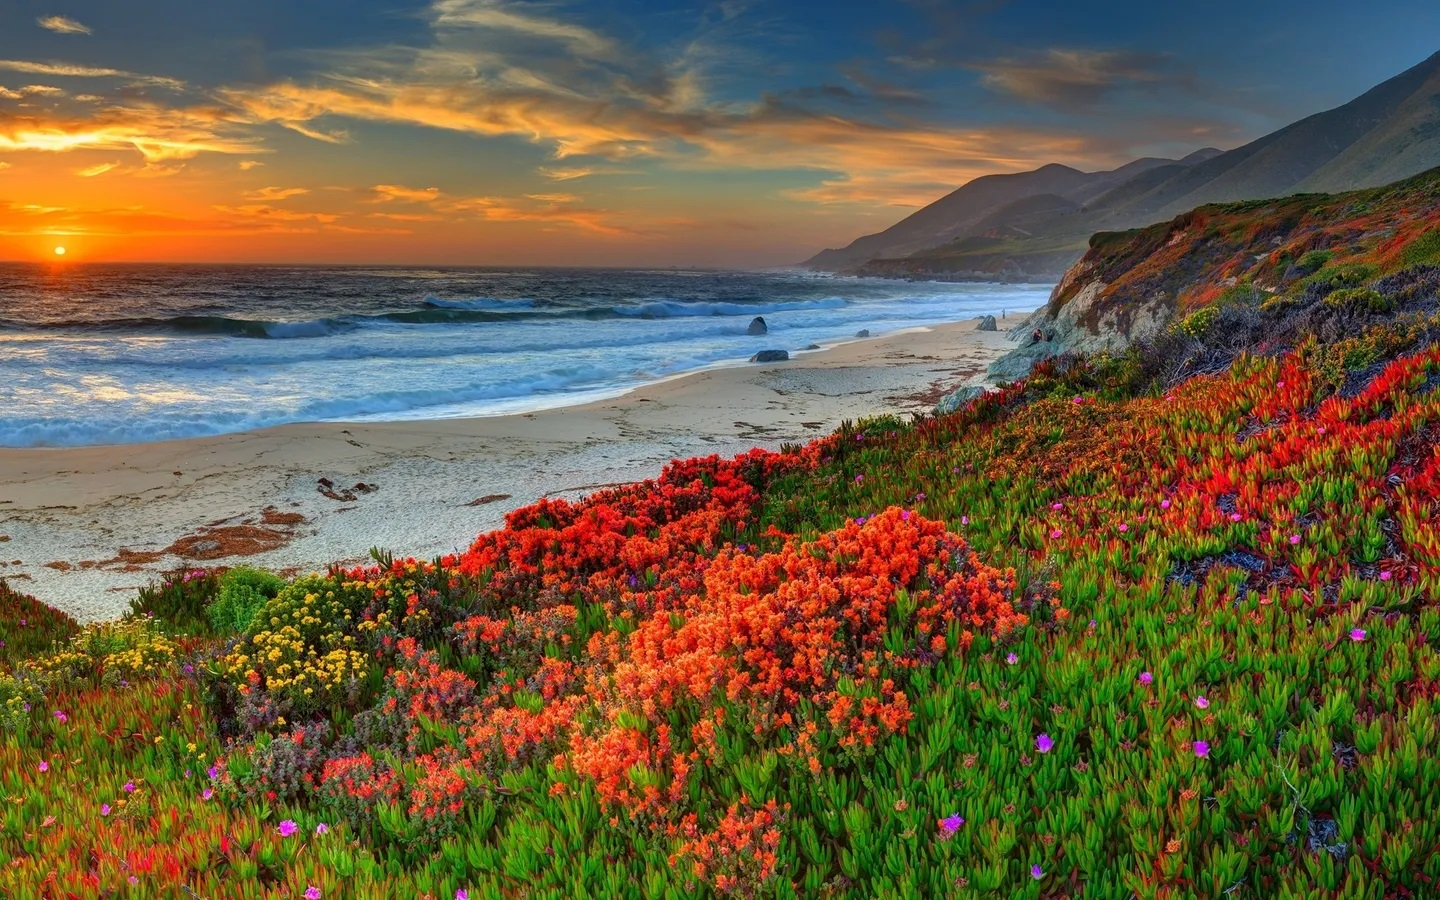
\includegraphics[width=0.9\textwidth]{figures/test.jpg}
    \caption{这里插入了一个普通的相片}
    \label{fig:my_pic1}
\end{figure}

\subsubsection{多图插图方法}
多图插图方法主要是用到subfloat来进行插图处理。
\begin{figure}[htbp]
    \begin{subfigure}[b]{0.4\textwidth}
        \centering
        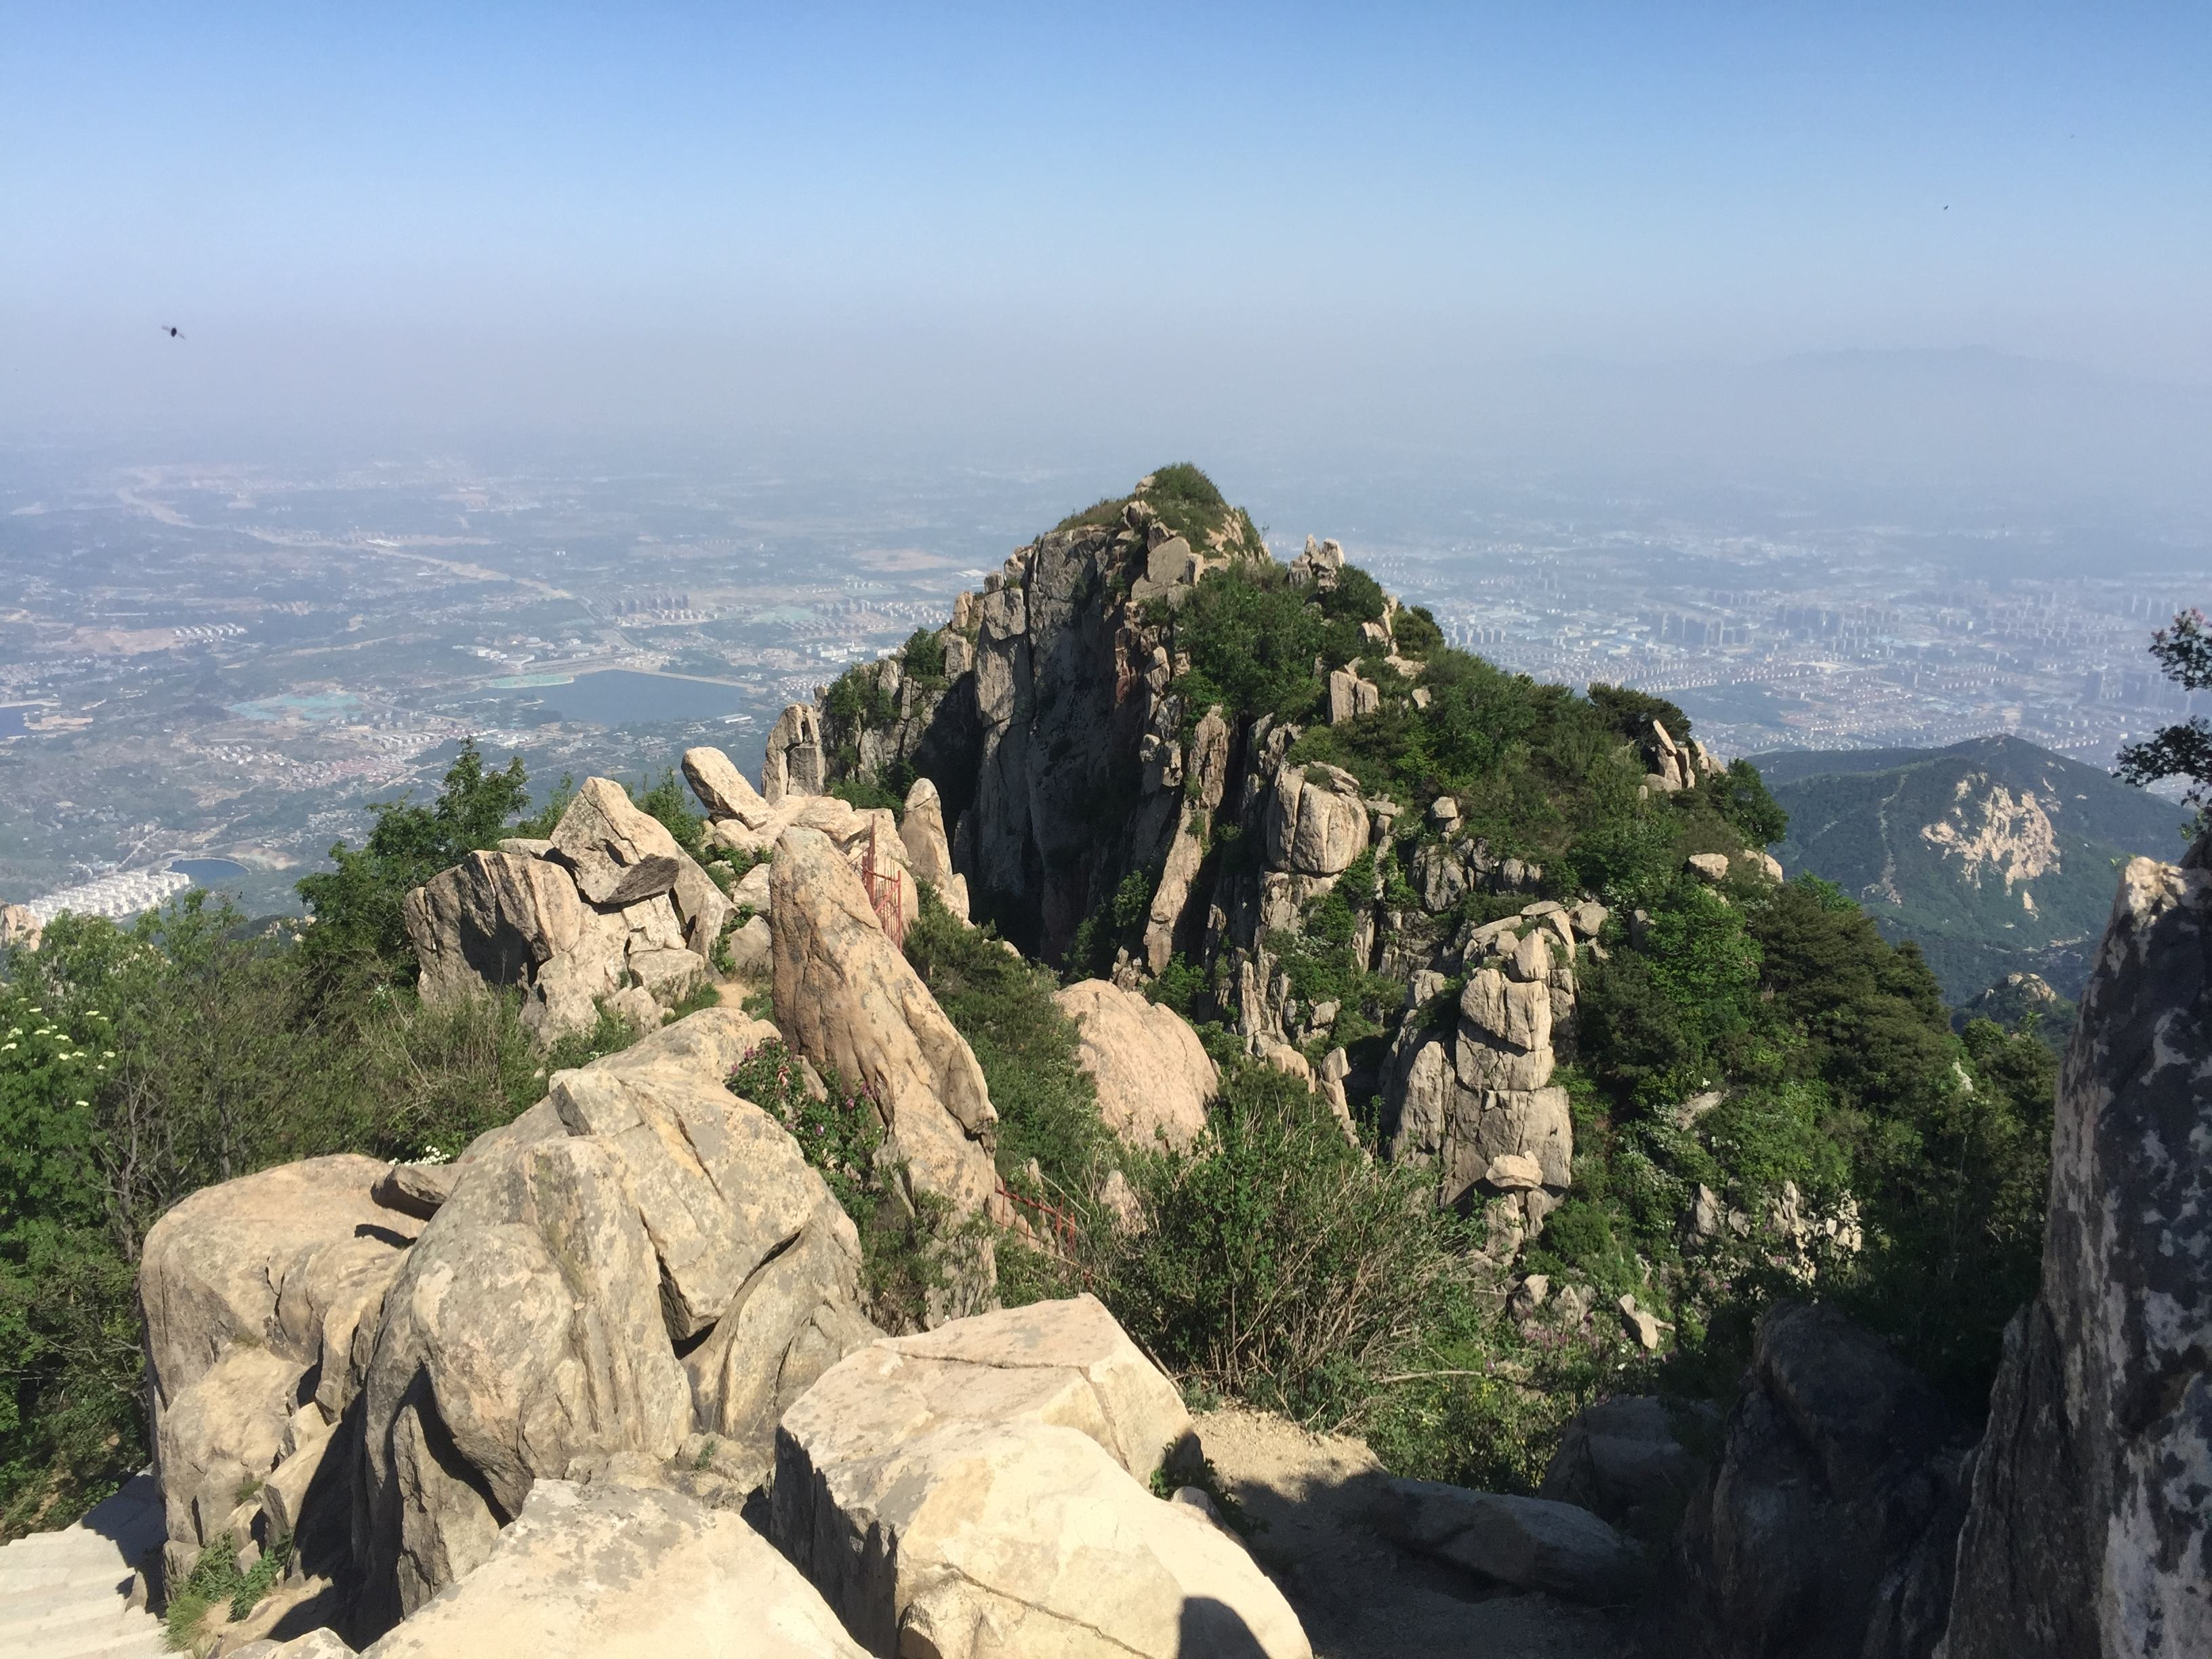
\includegraphics[width=\textwidth]{figures/taishan.jpeg}
        \caption{泰山}
        \label{fig:a}
    \end{subfigure}
    \begin{subfigure}[b]{0.4\textwidth}
        \centering
        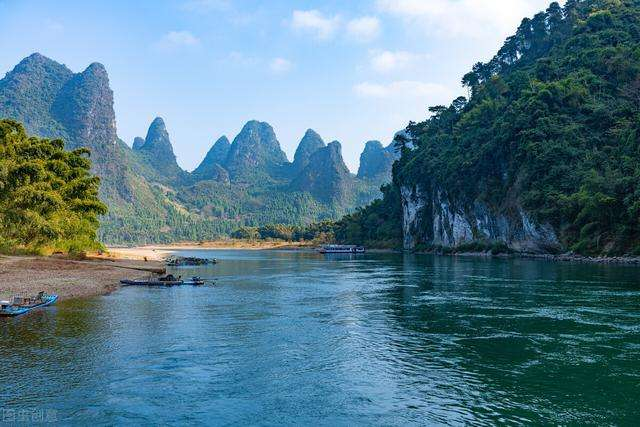
\includegraphics[width=\textwidth]{figures/guilin.jpeg}
        \caption{桂林山水}
        \label{fig:b}
    \end{subfigure}
    \quad
    \begin{subfigure}[b]{0.4\textwidth}
        \centering
        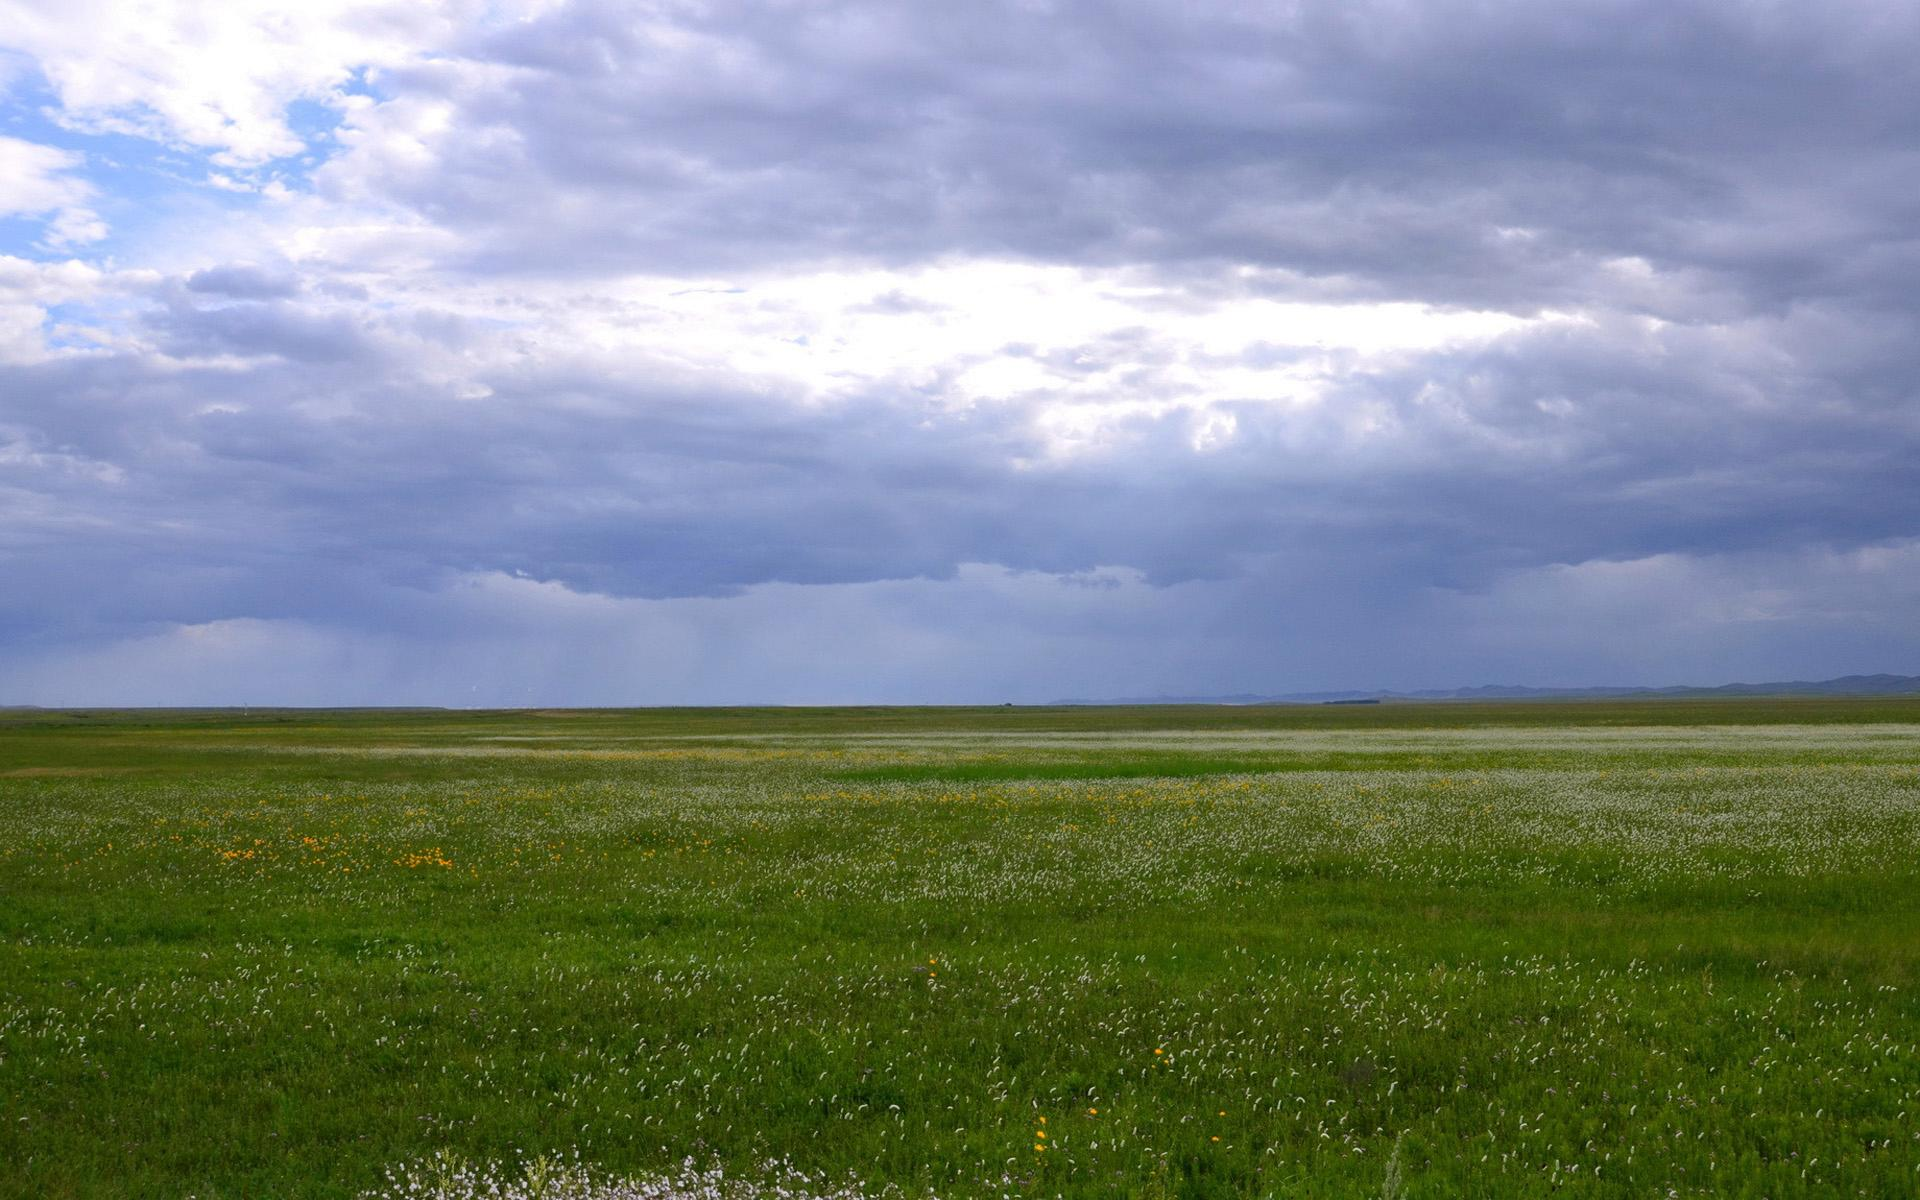
\includegraphics[width=\textwidth]{figures/xilinguole.jpeg}
        \caption{锡林郭勒盟草原}
        \label{fig:c}
    \end{subfigure}
    \begin{subfigure}[b]{0.4\textwidth}
        \centering
        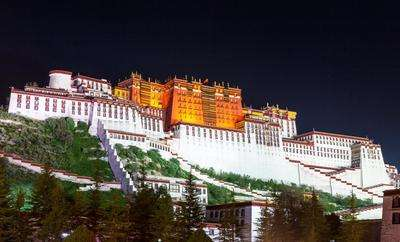
\includegraphics[width=\textwidth]{figures/budalagong.jpeg}
        \caption{布达拉宫}
        \label{fig:d}
    \end{subfigure}
    \centering
    \caption{示例的四张风景图片}
\end{figure}

\subsubsection{latex自带的一些插图方法}

另外一种就是latex自带的一种画图方法,这里示例两种latex自带的画图方法。
\begin{enumerate}
    \item \textbf{复杂网络结构图}:如图\ref{fig:complex_fig}(a) 所示。
    \item \textbf{函数图像}:如图\ref{fig:complex_fig}(b),(c) 所示,详细参考\href{https://pgfplots.sourceforge.net/gallery.html},函数图像的画法使用到的是pgfplots库当中的元素画图。
\end{enumerate}

\begin{figure}[hbpt]
    \centering
    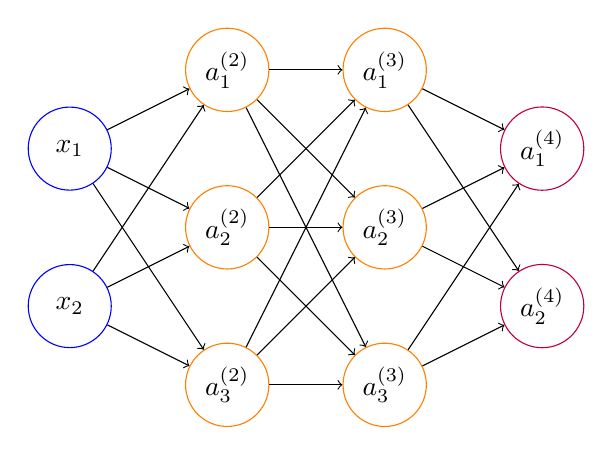
\begin{tikzpicture}
        \node[circle,
            minimum width =30pt ,
            minimum height =30pt ,draw=blue] (1) at(0,2){$x_1$};
        \node[circle,
            minimum width =30pt ,
            minimum height =30pt ,draw=blue] (2) at(0,0){$x_2$};
        \node[circle,
            minimum width =30pt ,
            minimum height =30pt ,draw=orange] (3) at(2,-1){$a_3^{(2)}$};
        \node[circle,
            minimum width =30pt ,
            minimum height =30pt ,draw=orange] (4) at(2,1){$a_2^{(2)}$};
        \node[circle,
            minimum width =30pt ,
            minimum height =30pt ,draw=orange] (5) at(2,3){$a_1^{(2)}$};
        \node[circle,
            minimum width =30pt ,
            minimum height =30pt ,draw=orange] (6) at(4,-1){$a_3^{(3)}$};
        \node[circle,
            minimum width =30pt ,
            minimum height =30pt ,draw=orange] (7) at(4,1){$a_2^{(3)}$};
        \node[circle,
            minimum width =30pt ,
            minimum height =30pt ,draw=orange] (8) at(4,3){$a_1^{(3)}$};
        \node[circle,
            minimum width =30pt ,
            minimum height =30pt ,draw=purple] (9) at(6,2){$a_1^{(4)}$};
        \node[circle,
            minimum width =30pt ,
            minimum height =30pt ,draw=purple] (10) at(6,0){$a_2^{(4)}$};
        \draw[->] (1) --(3);
        \draw[->] (1) --(4);
        \draw[->] (1) --(5);
        \draw[->] (2) --(3);
        \draw[->] (2) --(4);
        \draw[->] (2) --(5);
        \draw[->] (3) --(6);
        \draw[->] (3) --(7);
        \draw[->] (3) --(8);
        \draw[->] (4) --(6);
        \draw[->] (4) --(7);
        \draw[->] (4) --(8);
        \draw[->] (5) --(6);
        \draw[->] (5) --(7);
        \draw[->] (5) --(8);
        \draw[->] (6) --(9);
        \draw[->] (6) --(10);
        \draw[->] (7) --(9);
        \draw[->] (7) --(10);
        \draw[->] (8) --(9);
        \draw[->] (8) --(10);
    \end{tikzpicture}
    \caption{复杂网络结构图}
    \label{fig:complex_network}
\end{figure}

\begin{figure}
    \centering
    \subfloat[函数图像]{
        \begin{minipage}[t]{0.4\linewidth}
            \centering
            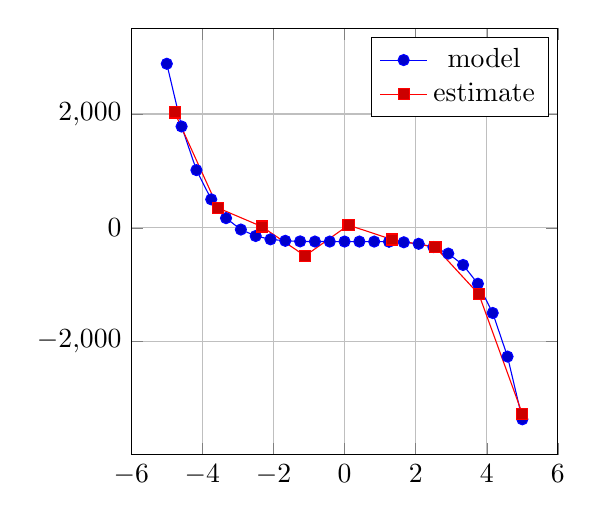
\begin{tikzpicture}
                \begin{axis}[
                    height=7cm,
                    width=7cm,
                    grid=major,
                ]
                    
                \addplot {-x^5 - 242};
                \addlegendentry{model}
            
                \addplot coordinates {
                    (-4.77778,2027.60977)
                    (-3.55556,347.84069)
                    (-2.33333,22.58953)
                    (-1.11111,-493.50066)
                    (0.11111,46.66082)
                    (1.33333,-205.56286)
                    (2.55556,-341.40638)
                    (3.77778,-1169.24780)
                    (5.00000,-3269.56775)
                };
                \addlegendentry{estimate}
                \end{axis}
            \end{tikzpicture}
        \end{minipage}
    }
    \subfloat[统计图]{
        \begin{minipage}[t]{0.4\linewidth}
            \centering
            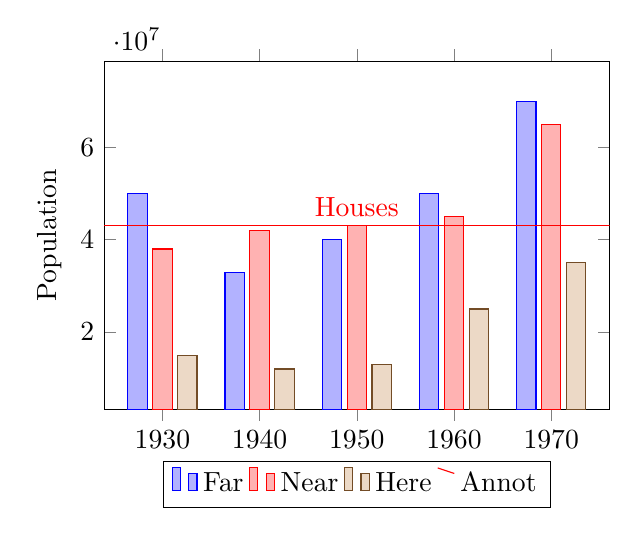
\begin{tikzpicture}
                \begin{axis}[
                    height=6cm,
                    width=8cm,
                    x tick label style={
                        /pgf/number format/1000 sep=},
                    ylabel=Population,
                    enlargelimits=0.15,
                    legend style={at={(0.5,-0.15)},
                        anchor=north,legend columns=-1},
                    ybar,
                    bar width=7pt,
                ]
                \addplot 
                    coordinates {(1930,50e6) (1940,33e6)
                         (1950,40e6) (1960,50e6) (1970,70e6)};
                
                \addplot 
                    coordinates {(1930,38e6) (1940,42e6) 
                        (1950,43e6) (1960,45e6) (1970,65e6)};
                
                \addplot 
                    coordinates {(1930,15e6) (1940,12e6) 
                        (1950,13e6) (1960,25e6) (1970,35e6)};
                
                \addplot[red,sharp plot,update limits=false] 
                    coordinates {(1910,4.3e7) (1990,4.3e7)} 
                    node[above] at (axis cs:1950,4.3e7) {Houses};
                
                \legend{Far,Near,Here,Annot}
                \end{axis}
            \end{tikzpicture}
        \end{minipage}
    }
    \caption{latex自带工具画图}
    \label{fig:complex_fig}
\end{figure}
